\chapter{Klassifikation}

Die Klassifikation besch\"aftigt sich mit der Einordnung von Objekten zu bestimmten Klassen. Die Objekte werden dabei durch einen sogenannten Merkmalsvektor \( x \in \mathbb{R}^n \) beschrieben, welcher definierte Eigenschaften des Objekts enth\"alt. Die benutzten Merkmale k\"onnen je nach Anwendungsfall unterschiedlich ausfallen. Im Bereich der Klassifikation von Verkehrsteilnehmern bieten sich geometrische Eigenschaften wie Ausma\ss{}e des Objekts, Umfang, Volumen oder Dichte an. Die zuzuordnende Klasse oder auch Label genannt ist im Allgemeinen eine ganze Zahl \(y \in \mathbb{Z} \). Der Klassifikator \(f\) l\"asst sich somit beschreiben als:

\begin{equation*}
 f: x \in \mathbb{R}^n \mapsto y \in \mathbb{Z}
\end{equation*}

Er ordnet den Merkmalen eines Objekts eine Klasse zu. Die Form des Klassifikators kann dabei variieren und h\"angt vom Anwendungsfall ab.
F\"ur gew\"ohnlich muss ein Klassifikator trainiert werden. Unter dem Begriff Training versteht man in diesem Zusammenhang den Vorgang, die w\"ahlbaren Parameter der Klassifikationsfunktion so einzustellen, dass er auf einen bestimmten Trainingsdatensatz \( (x_i | y_i)_{i=1..n} \) m\"oglichst gute Daten liefert. Das Training kann als Optimierungsproblem dargestellt werden:
\begin{equation*}
 \min_{\alpha} \sum_{i=1}^n \omega ( f_{\alpha}(x_i), y_i)
\end{equation*}
Die Funktion \( \omega : \mathbb{Z}^2 \mapsto \mathbb{R} \) ist eine Fehlerfunktion welche testet, ob die zu testende Klasse mit der vom Klassifikator ausgewerteten Klasse \"ubereinstimmt:
\begin{equation*}
 \omega (y_1, y_2) = 
 \begin{cases}
  0 & y_1=y_2 \\
  d(y_1, y_2) & y_1 \neq y_2, d>0
 \end{cases}
\end{equation*}

Durch Minimierung der Summe der Fehler kann so eine bestm\"ogliche Approximation an die Trainingsdaten gefunden werden. Im Folgenden werden einige Klassifikatoinsverfahren vorgestellt.

\section{K-Nearest-Neighbor Klassifikation}
Der Nearest-Neighbor-Klassifikator arbeitet ohne einen Optimiegunssprozess direkt auf den Trainingsdaten \( (x_i | y_i)_{i=1..m} \in \mathbb{R}^n \times \mathbb{Z} \). Ein Objekt mit Merkmalen \(b \in \mathbb{R}^n\) wird derjenigen Klasse zugeordnet, zu der der Abstand \(d=\|b-x_i\| \) am geringsten ist:
\begin{equation*}
 f(b)= y_k, k=\underset{{k \in \{1..m\}}}{arg\,min} (||b-x_k||)
\end{equation*}

Die Norm \(\| \cdot \| \) ist hierbei beliebig, h\"aufig wird jedoch die euklidische Norm \(\| \cdot \|_2 \) verwendet.

In Abbildung \ref{fig:classification_knn} ist ein Beispiel f\"ur eine solche Klassifikation zu sehen. Auf der linken Seite wird ein einfacher Nearest-Neighbor-Klassifikator angewendet. Auf der rechten Seite ist jedoch sichtbar, dass das Rauschen in den Daten zu einer Fehlklassifikation f\"uhren w\"urde. Aus diesem Grund wurde der Klassifikator erweitert zum K-Nearest-Neighbor-Klassifikator. Dieser bezieht nicht nur das Trainingsdatum mit dem geringsten Abstand ein, sondern sucht die \(k\) n\"achsten Nachbarn. Das Ergebnis der Klassifikation ist dann diejenige Klasse, welche am h\"aufigsten in dieser Ergebnismenge vorkommt. In der Grafik ist der KNN-Klassifikator f\"ur den fall \(k=3\) dargestellt.

Der KNN-Klassifikator finden h\"aufig zu Testzwecken Anwendung, da er einfach zu implementieren ist und stabile Resultate liefert. Da er kein Training ben\"otigt ist jedoch der Aufwand zur Evaluation hoch und der Algorithmus ist damit nicht sehr effizient. Zu produktiven Zwecken in Echtzeitsystemen wird er daher nur selten verwendet.

\begin{figure}
 \centering
 \includegraphics[width=1\textwidth]{media/classification/knn_example.png}
 \caption{Klassifikation - Beispiel f\"ur NN- und KNN-Klassifikator}
 \label{fig:classification_knn}
\end{figure}

\section{Neuronales Netz}
K\"unstliche neuronale Netze sind Modelle, welche biologischen neuronalen Netzen nachempfunden sind. Sie setzen sich aus einer Vielzahl von Neuronen zusammen, welche untereinander verbunden sind und sich gegenseitig beeinflussen bzw. anregen k\"onnen. Ein k\"unstliches neuronales Netz besteht aus einer Eingabeschicht, einem oder mehreren Zwischenschichten und einer Ausgabeschicht. Ein Modell eines solchen Netzes mit einer Zwischenschicht ist in Abbildung \ref{fig:classification_neuralnetwork} zu sehen. Die Eingabeschicht akzeptiert hierbei \(m=4\) Daten als Eingabe, die Zwischenschicht besteht aus \(5\) k\"unstlichen Neuronen und die Ausgabeschicht  liefert ein Ergebnis aus \(n=3\) Ausgabedaten.

\begin{figure}
\centering
\def\layersep{3cm}
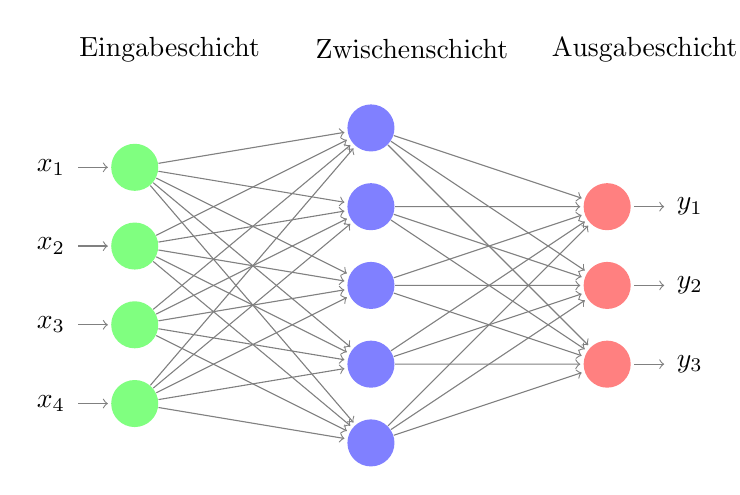
\begin{tikzpicture}[shorten >=1pt,->,draw=black!50, node distance=\layersep]
    \tikzstyle{every pin edge}=[<-,shorten <=1pt]
    \tikzstyle{neuron}=[circle,fill=black!25,minimum size=17pt,inner sep=0pt]
    \tikzstyle{input neuron}=[neuron, fill=green!50];
    \tikzstyle{output neuron}=[neuron, fill=red!50];
    \tikzstyle{hidden neuron}=[neuron, fill=blue!50];
    \tikzstyle{annot} = [text width=4em, text centered]

    % Draw the input layer nodes
    \foreach \name / \y in {1,...,4}
    % This is the same as writing \foreach \name / \y in {1/1,2/2,3/3,4/4}
        \node[input neuron, pin=left:\(x_\y\)] (I-\name) at (0,-\y) {};

    % Draw the hidden layer nodes
    \foreach \name / \y in {1,...,5}
        \path[yshift=0.5cm]
            node[hidden neuron] (H-\name) at (\layersep,-\y cm) {};
            
    % Draw the output layer node
    %\node[output neuron,pin={[pin edge={->}]right:y1}, right of=H-3] (O) {};
    \foreach \name / \y in {1,...,3}
        \node[output neuron, pin={[pin edge={->}]right:\(y_\y \)}] (O-\name) at (2*\layersep,-\y-0.5) {};

    % Connect every node in the input layer with every node in the
    % hidden layer.
    \foreach \source in {1,...,4}
        \foreach \dest in {1,...,5}
            \path (I-\source) edge (H-\dest);

    % Connect every node in the hidden layer with the output layer
    \foreach \source in {1,...,5}
        \foreach \dest in {1,...,3}
            \path (H-\source) edge (O-\dest);

    % Annotate the layers
    \node[annot,above of=H-1, node distance=1cm] (hl) {Zwischenschicht};
    \node[annot,left of=hl] {Eingabeschicht};
    \node[annot,right of=hl] {Ausgabeschicht};
\end{tikzpicture}
\caption{Modell eines k\"unstlichen neuronalen Netzes mit einer Zwischenschicht}
\label{fig:classification_neuralnetwork}
\end{figure}

Das Single-Layer-Perzeptron ist das primitivste Netz, welches gebildet werden kann. Es besteht lediglich aus einer Eingabe- und einer Ausgabeschicht. Die Funktion l\"asst sich also wie folgt formulieren:

\begin{equation}
 f_W(x)=\varphi(W \cdot x)
\end{equation}
Der Vektor \(x \in \mathbb{R}^m \) beschreibt die Eingabedaten, die Matrix \(W \in \mathbb{R}^{n \times m} \) enth\"alt die Gewichte der Verbindungen zwischen den Neuronen und die Funktion \(\varphi \) ist die sogenannte Aktivierungsfunktion eines Neurons. Die Aktivierungsfunktion eines Neurons entscheidet, ab welchem Wert ein Neuron angeregt ist oder nicht. Hierbei k\"onnen unterschiedliche Funktionen eingesetzt werden: \\
\begin{tabular}{ll}
 S\"attigungsfunktion & \( \varphi(z)=
\begin{cases}
 0 & z \leq -a \\
 \frac{z}{2a} & -a \leq z \leq a, a \in \mathbb{R} \\
 1 & a \leq z
\end{cases}
\) \\
Fermi-Funktion & \( \varphi(z)=\frac{1}{1+e^{\frac{-z}{a}} }, a \in \mathbb{R} \) \\
Heavyside-Funktion & \(\varphi(z)=
\begin{cases}
 0 & z<0 \\
 1 & z\geq 0
\end{cases} \) \\
Lineare Funktion & \( \varphi(z) = a \cdot z \)
\end{tabular}

Im Allgemeinen wird vorausgesetzt, dass alle Neuronen einer Schickt die gleiche Aktivierungsfunktion besitzen.
F\"ur gew\"ohnlich bestehen neuronale Netze aus mehreren Schichten Perzeptronen. Die einzelnen Ergebnisse der Schichten werden nun nacheinander verkn\"upft um so das Ergebnis der Ausgabeschicht zu erhalten:
\begin{equation}
 f_W(x) = \varphi_k(W_k \cdot \varphi_{k-1}(W_{k-1} \cdot \varphi_{k-2}(... \cdot \varphi_1(W_1x)...)))
\end{equation}
Die Matrizen \(W_k\) repr\"asentieren hierbei die Gewichte der Kanten der einzelnen Schichten. Die Gr\"o\ss{}e h\"angt als von der Anzahl der Neuronen in der jeweiligen Schicht ab. Ebenso kann sich die Aktivierungsfunktion \( \varphi_k\) der einzelnen Schichten unterscheiden.

Beim Training eines neuronalen Netzes werden die Gewichte \(W_k\) bestimmt. Hierzu ist wiederum ein Trainingsdatensatz notwendig: 
 \( (x_k | y_k)_{k=1..r} \in \mathbb{R}^m \times \mathbb{R}^n \)
Der eigentliche Trainigsvorgang soll die Gewichte so bestimmen, dass der quadratische Fehler der Klassifikation minimiert wird:
\begin{equation}
 \underset{W}{min} \sum_{k=1}^r \sum_{j=1}^n (f_W(x_j^k)-y_j^k)^2
\end{equation}
Hierbei handelt es sich um ein unrestringiertes Optimierungsproblem, da an die zu optimierende Variable \(W\) keine Nebenbedingungen gekn\"upft sind. Zum L\"osen des Optimierungsproblems existieren diverse Verfahren. Welches Verfahren eingesetzt wird h\"angt von der Zusammensetzung des Netzes und der Wahl der Aktivierungsfunktion zusammen. Ist die resultierende Funktion linear k\"onnen schnellere Verfahren wie die QR-Zerlegung oder das CG-Verfahren eingesetzt werden. Im nichtlinearen Fall sind m\"ogliche Verfahren das Gradientenverfahren, das Newtonverfahren oder auch das Levenberg-Marquardt-Verfahren.

\section{Support Vector Machine}
Die Klassifikation durch die sogenannte Support Vector Machine wird vorallem f\"ur bin\"are Klassifikationsprobleme verwendet. Ziel der Methode ist es, eine Hyperebene zu finden, welche zwei linear trennbare Mengen voneinander trennt. Der Klassifikator hat die Form
\begin{equation*}
 f_{w, b}(x) = 
 \begin{cases}
  1 & w^\intercal x+b>0 \\
  0 & sonst
 \end{cases}
\end{equation*}
 Der Vektor \(w \in \mathbb{R}^n \) ist die Normale der Ebene, das Skalar \(b \in \mathbb{R}\) ist der sogenannte Bias, also die Verschiebung. Diese beiden Parameter m\"ussen durch das Training des Klassifikators berechnet werden. Hierzu wird das Optimierungsproblem anhand der Trainingsdaten \( (x_i | y_i)_{i=1..m} \in \mathbb{R}^n \times \mathbb{Z} \) formuliert:
\begin{eqnarray*}
 & \min \frac{1}{2}||w||_2^2 \\
 & y_i(w^\intercal x_i+b) \geq 1, \forall (x_i | y_i)
\end{eqnarray*}
Die Nebenbedingung fordert hierbei, dass beide Klassen tats\"achlich linear trennbar sind. Da dies im Allgemeinen nicht der Fall ist wird eine sogenannte Schlupfvariable eingef\"ugt, welche die Verletzung der Nebenbedingung erlaubt:
\begin{eqnarray*}
 &\min \frac{1}{2}||w||_2^2+C \sum_{i=1}^m \xi_i \\
 &y_i(w^\intercal x_i+b) \geq 1-\xi_i, \forall (x_i | y_i)
\end{eqnarray*}

In Abbildung \ref{fig:classification_svmlinear} ist eine lineare Trennebene zu sehen. Die Methode der Support Vector Machine erm\"oglicht neben einer linearen auch eine nichtlineare Trennebene, was in Abbildung \ref{fig:classification_svmnonlinear} zu sehen ist. Das Optimierungsproblem gestaltet sich dabei deutlich komplexer, weshalb in dieser Arbeit auf die lineare Variante zur\"uckgegriffen wird.

\begin{figure}
\centering
\begin{minipage}{.5\textwidth}
  \centering
  \includegraphics[width=1\textwidth]{media/classification/svm_linear.png}
  \captionof{figure}{SVM linear}
  \label{fig:classification_svmlinear}
\end{minipage}%
\begin{minipage}{.5\textwidth}
  \centering
  \includegraphics[width=1\textwidth]{media/classification/svm_nonlinear.png}
  \captionof{figure}{SVM nichtlinear}
  \label{fig:classification_svmnonlinear}
\end{minipage}
\end{figure}
